\clearpage
\section[An analyze of a raw material for \moha\ related memes]{An analyze of a raw material for {\sc m\'o-h\'a}\ related memes}
\label{script}
This appendix includes the script of the video of Jiang Zemin angrily chastised a Hong Kong journalist i.e.\ \smallcaps{video 1}, transcribed and translated by the author based on the original Chinese subtitle, with minor adjustments. This video is chosen as an example here because it is the best known and most widely used material for creation of memes related to the \moha\ subculture.
\begin{marginfigure}
	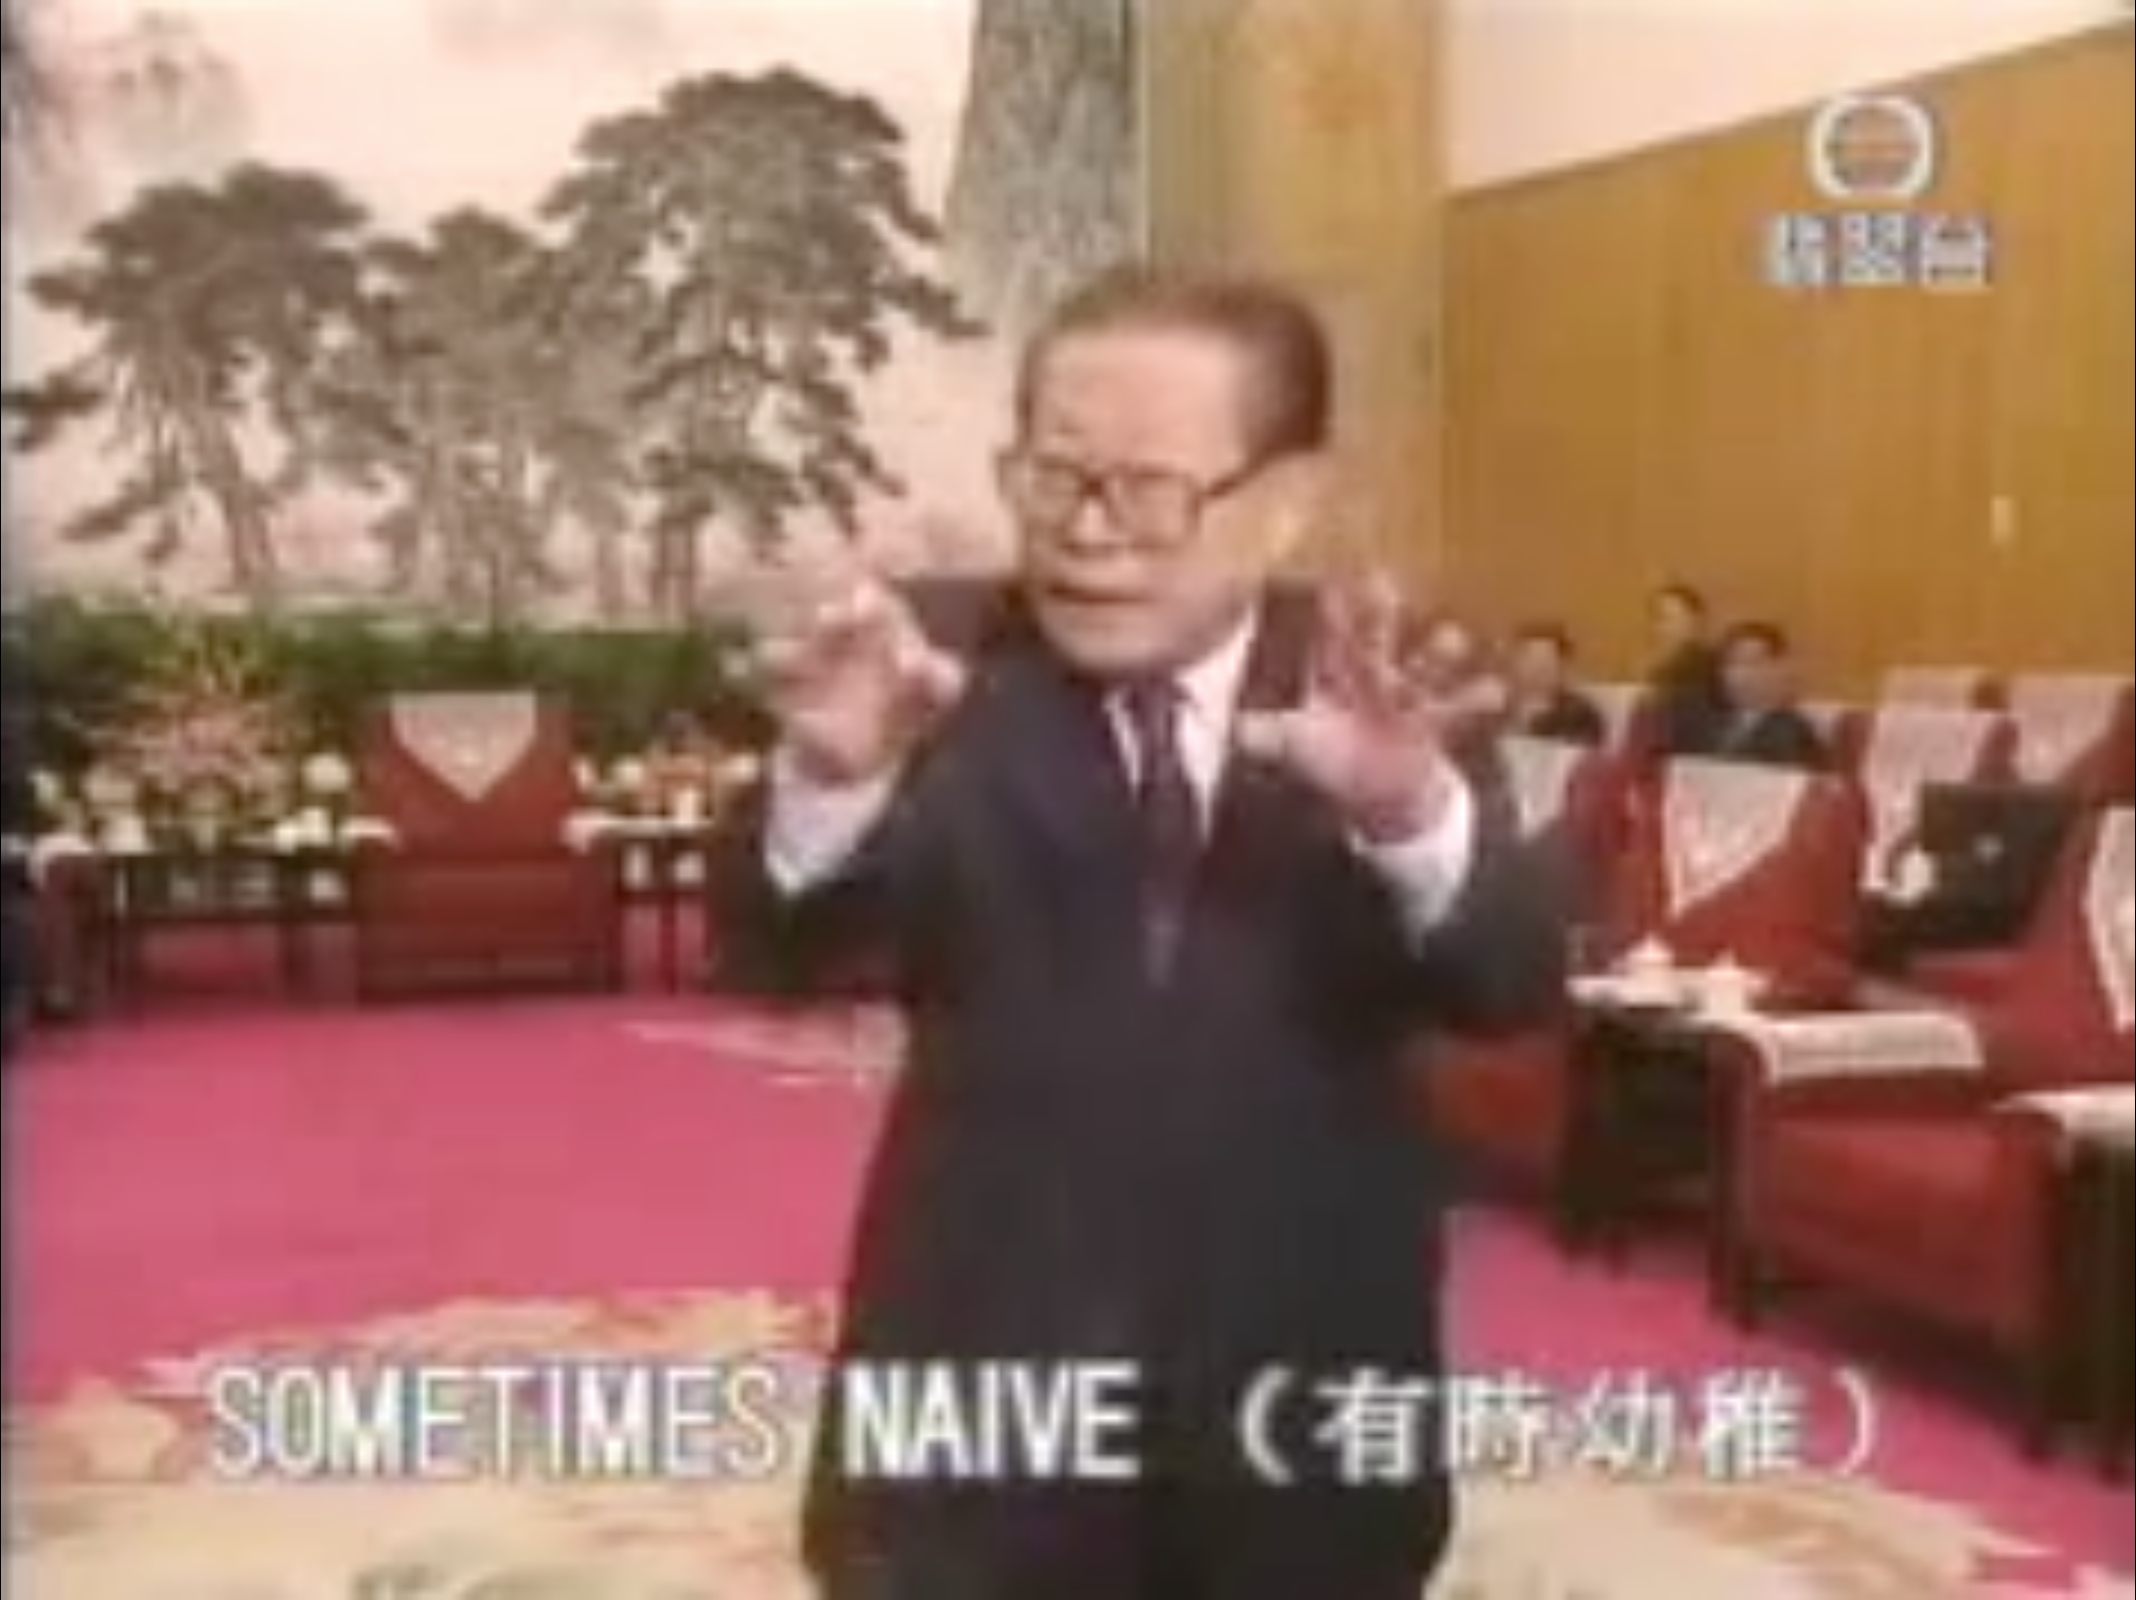
\includegraphics[width=\textwidth]{video1.png}
	\caption[A screenshot from \smallcaps{video 1}]{A screenshot from \smallcaps{video 1}. Souce: \url{https://youtu.be/NsGbhDVFxQw}, at 3:25.}
\end{marginfigure}
All phrases underlined in the script are being used for creating memes, some for its content and some for its tone when it was said by Jiang. Phrases that are italicized (for the Chinese part, the Kai-type font is used as equivalent) and marked with ``\cann'' are said in Cantonese. Some phrases is said directly in English, which could be read from the script, are also italicized. \smallcaps{jo} refers to the journalist, and \smallcaps{ji} refers to Jiang Zemin.
\ex[glhangstyle=none, everygla=\rm, exnoformat=X:, exno={\smallcaps{jo}}, belowexskip=0pt]
\begingl
\gla
{江主席,} {你觉得} {董先生} {连任} {好不好呀?}//
\glb
{President Jiang,} {do you think} {Mr.\ Tung} {serving a second term} {is a good idea?}//
\endgl
\xe
\ex[glhangstyle=none, everygla=\rm, exnoformat=X:, exno={\smallcaps{ji}}, belowexskip=0pt, aboveexskip=-.5cm]
\begingl
\gla
{\it \underline{好呀}!\rm \cann} {}//
\glb
{\textit{It is}!} {}//
\endgl
\xe
\ex[glhangstyle=none, everygla=\rm, exnoformat=X:, exno={\smallcaps{jo}}, belowexskip=0pt, aboveexskip=-.5cm]
\begingl
\gla
{} {中央} {也} {支持他吗?}//
\glb
{[Does]} {Beijing (the Cental)} {also} {support this (him)?}//
\endgl
\xe
\ex[glhangstyle=none, everygla=\rm, exnoformat=X:, exno={\smallcaps{ji}}, belowexskip=0pt, aboveexskip=-.5cm]
\begingl
\gla
{当然啦!} {}//
\glb
{Of course!} {}//
\endgl
\xe
\ex[glhangstyle=none, everygla=\rm, exnoformat=X:, exno={\smallcaps{jo}}, belowexskip=0pt, aboveexskip=-.5cm]
\begingl
\gla
{为什么} {那么早就提出?} {是否} {没有} {别的人选?} //
\glb
{Why} {put this forward this early?} {Is it because} {there is no} {other [suitable] candidate?}//
\endgl
\xe
\ex[glhangstyle=none, everygla=\rm, exnoformat=X:, exno={\smallcaps{ji}}, belowexskip=0pt, aboveexskip=-.5cm]
\begingl
\gla
{我} {没有} {时间} {} {跟你们谈。}//
\glb
{I} {don't have} {time} {to} {talk about this with you.}//
\endgl
\xe
\ex[glhangstyle=none, everygla=\rm, exnoformat=X:, exno={\smallcaps{jo}}, belowexskip=0pt, aboveexskip=-.5cm]
\begingl
\gla
{江主席,} {欧盟} {最近} {发表了} {一个} {报告,} {说} {北京} {会透过一些渠道} {去影响} {、} {干预} {香港的法治,} {你对这个看法有什么回应呢?}//
\glb
{President Jiang,} {the \smallcaps{eu}} {recently} {released} {a} {report,} {claiming that} {Beijing} {will use some channel} {to influence} {and} {intervene} {the rule of law in Hong Kong,} {what's your response to this opinion?}//
\endgl
\xe
\ex[glhangstyle=none, everygla=\rm, exnoformat=X:, exno={\smallcaps{ji}}, belowexskip=0pt, aboveexskip=-.5cm]
\begingl
\gla
{没听过} {}//
\glb
{I never heard about that.} {}//
\endgl
\xe
\ex[glhangstyle=none, everygla=\rm, exnoformat=X:, exno={\smallcaps{jo}}, belowexskip=0pt, aboveexskip=-.5cm]
\begingl
\gla
{是} {彭定康说的。}//
\glb
{It is} {Chris Patten[1]'s word.}//
\glft[] [1] Chris Patten was the last British Governor of Hong Kong, one of the \smallcaps{uk}'s two members of the European Commission at the time.//
\endgl
\xe
\ex[glhangstyle=none, everygla=\rm, exnoformat=X:, exno={\smallcaps{ji}}, belowexskip=0pt, aboveexskip=-.5cm]
\begingl
\gla
{你们} {媒体} {千万要} {记着,} {不要} {\underline{「见得风,是得雨」[2]}。} {接到这些} {消息,} {你媒体} {本身也要判断,} {明白我的意思吗?} {假使} {\underline{这些完全无中生有的东西,}} {\underline{你再帮他说一遍,}} {\underline{你等于$\ldots$你也有责任吧?}}//
\glb
{You} {media} {must} {remember,} {don't} {``see wind as rain''.} {When getting these} {news,} {you media} {have to make your own judgement,} {you know what I mean?} {If} {something coming out of thin air,} {you keep repeating it,} {you should also take responsibility for it, don't you?}//
\glft[] [2] This is a Chinese idiom, literally means ``hear the wind and claim there is rain'', used to describe those who easily believe something with only a little evidence or hearsay.//
\endgl
\xe
\ex[glhangstyle=none, everygla=\rm, exnoformat=X:, exno={\smallcaps{jo}}, belowexskip=0pt, aboveexskip=-.5cm]
\begingl
\gla
{现在那么早,} {你们就是说支持} {董先生,} {\underline{会不会给人}} {\underline{一种感觉,}} {\underline{就是内定了、钦点了董先生呢?}}//
\glb
{Now it is still early} {but you already showing support to} {Mr.\ Tung,} {will this give people} {a feeling,} {that Mr.\ Tung is selected by imperial order?}//
\endgl
\xe
\ex[glhangstyle=none, everygla=\rm, exnoformat=X:, exno={\smallcaps{ji}}, belowexskip=0pt, aboveexskip=-.5cm]
\begingl
\gla
{} {\underline{没有任何这个的意思。}} {} {还是按照} {香港的$\ldots$} {\underline{按照基本法}、} {按照选举法---} {去产生} {$\ldots\ldots$}//
\glb
{[I]} {didn't mean that at all.} {[The election]} {will still follow} {Hong Kong's$\ldots$} {Basic Law,} {the Election Law---} {to produce} {(the result$\ldots$)}//
\endgl
\xe
\ex[glhangstyle=none, everygla=\rm, exnoformat=X:, exno={\smallcaps{jo}}, belowexskip=0pt, aboveexskip=-.5cm]
\begingl
\gla
{但是} {你们$\ldots$}//
\glb
{But} {you$\ldots$}//
\endgl
\xe
\ex[glhangstyle=none, everygla=\rm, exnoformat=X:, exno={\smallcaps{ji}}, belowexskip=0pt, aboveexskip=-.5cm]
\begingl
\gla
{刚才你问我啊,} {\underline{我可以}} {\underline{回答你一句}} {\underline{「无可奉告」},} {那你们又不高兴,} {那怎么办?} {我的意思不是} {我是} {钦点} {他当下一任。} {你问我} {支持不支持,} {我是支持的。} {我就明确地给你告诉这一点。} {我觉得} {你们啊$\ldots$} {我感觉} {你们新闻界} {还要学习一个,} {你们} {非常} {熟悉} { 西方的这一套理论。 } {你们毕竟还} {\textit{\underline{too young}},} {明白这意思吧?} {我告诉你们} {\underline{我是身经百战了,}} {\underline{见得多了!}} {\underline{西方的哪一个国家}} {\underline{我没去过?}} {你们要知道,} {\underline{美国的华莱士,}} {\underline{比你们不知道高到哪里去了,}} {\underline{我跟他谈笑风生。}} {所以说媒体啊,} {\underline{还是要提高}} {\underline{自己的知识水平,}} {\textit{\underline{识得唔识得啊}} \cann?} {我也给你们着急啊,} {真的。} {\underline{你们}} {\underline{有}} {\underline{一个}} {\underline{好,}} {\underline{全世界跑到什么地方,}} {\underline{你们比其他的西方记者跑得还快。}} {但是呢,} {问来问去的问题啊,} {都} {\textit{\underline{too simple}},} {\underline{\textit{sometimes na\"{i}ve}!}} {懂了没有啊?}//
\glb
{What you just ask me,} {I could} {just say} {``no comment'',} {but that will then make you unhappy,} {what should I do?} {I didn't mean} {I am} {making an imperial order} {to make him serve another term.} {If you ask me} {support it or not,} {I support it.} {I can tell you this clearly.} {I think} {you$\ldots$} {I think} {you field of journalism} {still have to learn more,} {you are} {very} {familiar with} {western theories,} {but you are still} {\textit{too young},} {you understand?} {I tell you,} {I have experienced many battles,} {I have seen a lot!} {Which western country} {haven't I been?} {You know,} {the Wallace from the \usa,} {he was way better than you,} {and I talked with him cheerfully and smoothly.} {So you media,} {should improve} {your level of knowledge,} {\textit{do you understand}?} {I'm worrying about you,} {really.} {You} {have} {one} {advantage,} {you run all around the world,} {even faster than other western journalists.} {But} {the questions you ask,} {are all} {\textit{too simple},} {\textit{sometimes na\"{i}ve}!} {Do you understand?}//
\endgl
\xe
\ex[glhangstyle=none, everygla=\rm, exnoformat=X:, exno={\smallcaps{jo}}, belowexskip=0pt, aboveexskip=-.5cm]
\begingl
\gla
{但是} {能不能说一下} {为什么} {支持董建华呢?}//
\glb
{But} {can you explain} {why} {you support Tung Chee-hwa?}//
\endgl
\xe
\ex[glhangstyle=none, everygla=\rm, exnoformat=X:, exno={\smallcaps{ji}}, belowexskip=0pt, aboveexskip=-.5cm]
\begingl
\gla
{我很抱歉,} {我今天是\underline{作为一个长者}跟你们讲的。} {我} {不是} {新闻工作者,} {但是} {我} {见得太多了,} {\underline{我}} {\underline{有必要}} {\underline{告诉你们一点}} {\underline{人生的经验。}} {刚才} {我很想啊,} {就是我每一次碰到你们,} {我就讲} {中国} {有一句话叫} {\underline{「闷声大发财」},} {我就} {\underline{什么话也不说。}} {\underline{这}} {\underline{是}} {\underline{最好的!}} {但是} {我想,} {我见到你们这样热情啊,} {一句话不说也不好。} {所以} {你刚才} {一定要---} {\underline{在宣传上将来如果你们报道上有偏差,}} {\underline{你们要负责的。}} {我} {没有说} {要钦定,} {没有任何这个意思。} {但是} {你} {一定要} {问我,} {对董先生支持不支持,} {我们不支持他?} {他} {现在是} {特首,} {我们怎么能不支持} {特首?}//
\glb
{My apology,} {today I'm talking to you as an elder.} {I} {am not} {an journalism practitioner,} {but} {I} {have seen a lot.} {I} {am responsible} {to tell you some} {experiences of life.} {Just now} {I really want to,} {every time I see you,} {I (want to) say} {in China} {we have an old saying,} {``remain silent and make big fortune'',} {I} {don't say anything,} {this} {is} {the best!} {But} {I was thinking,} {you have such an enthusiasm,} {it is not nice if I don't say a word.} {So} {just now you} {insist---} {if there is anything inaccurate in your news report,} {you have to take the responsibility.} {I} {didn't say} {we are making an imperial order,} {not at all.} {But} {if you} {insist to} {ask me,} {if I support Mr.\ Tung or not,} {how could we not support him?} {He} {is the current} {chief executive,} {how could we not support} { the chief executive? }//
\endgl
\xe
\ex[glhangstyle=none, everygla=\rm, exnoformat=X:, exno={\smallcaps{jo}}, belowexskip=0pt, aboveexskip=-.5cm]
\begingl
\gla
{但是} {如果说} {连任呢?}//
\glb
{But} {what if} {serving another term?}//
\endgl
\xe
\ex[glhangstyle=none, everygla=\rm, exnoformat=X:, exno={\smallcaps{ji}}, belowexskip=0pt, aboveexskip=-.5cm]
\begingl
\gla
{连任} {也要} {按照} {香港的法律啊,} {对不对?} {要按照} {香港的$\ldots$} {\underline{当然}} {\underline{我们的决定权}} {\underline{也是}} {\underline{很}} {\underline{重要的。}} {香港特别行政区} {是属于} {中国$\ldots$} {中华人民共和国的中央人民政府啊。} {到那个时候我们会表态的!} {明白我这意思吧?} {\underline{你们啊,}} {\underline{不要想}} {\underline{弄个}} {\underline{大新闻,}} {\underline{说}} {\underline{现在已经钦定了,}} {\underline{再把我批判一番。}} {\underline{你们啊,}} {\underline{\textit{na\"{i}ve}!}} {\underline{\textit{I'm angry}!}} {我跟你讲,} {你们这样子啊,} {是不行的!}//
\glb
{The succession} {will also} {follow} {the laws in Hong Kong,} {won't it?} {Follow} {Hong Kong's$\ldots$} {of course} {our (Beijing's) right of decision} {is also} {very} {important.} {The Hong Kong Special Administrative Region} {belongs to} {China$\ldots$} {the Central People's Government of the People's Republic of China.} {We will make our declaration by then.} {You know what I mean?} {You (media),} {do not try to} {make a} {big news,} {saying something like} {``imperial order'',} {then [use it to] criticize me.} {You,} {\textit{na\"{i}ve}!} {\textit{I'm angry}!} {I tell you,} {acting like this,} {does not work!}//
\endgl
\xe



